\subsection{La question}
Le joueur au trait cherche-t-il seulement à minimiser l'énergie (jouer le meilleur coup), ou tient-il aussi compte
du \emph{nombre d'options} que laisse chaque coup ? Pour un coup $i$, on évalue (Stockfish, profondeur 10) :
\begin{itemize}
  \item la position \emph{fille} (adversaire au trait) : $S_\text{adv}(i) = \log N_\text{bons}$, où $N_\text{bons}$
        est le nombre de coups de l'adversaire à moins de 50 cp de son meilleur ;
  \item la position \emph{petite-fille}, après la meilleure réponse adverse : $S_\text{moi}(i)$, même définition
        pour le joueur.
\end{itemize}
$S$ est une entropie de Boltzmann, $S = \log(\text{nombre d'états accessibles})$. Garder $S_\text{moi}$ élevé,
c'est garder des options (jeu \og stratégique\fg{}) ; rendre $S_\text{adv}$ faible, c'est forcer l'adversaire à
trouver le seul bon coup (jeu \og tactique\fg{}).

\subsection{Deux modèles}
\paragraph{(A) Compromis énergie / entropie.} On ajoute l'entropie à l'« utilité » de chaque coup :
\begin{equation}
  p_i \propto \exp\!\Big[-\big(\DE_i/s\big)^{c} + \lambda_\text{moi}\, S_\text{moi}(i) + \lambda_\text{adv}\, S_\text{adv}(i)\Big].
\end{equation}
C'est l'analogue d'une \textbf{énergie libre} $F_i = E_i - \tau S_i$ : $\lambda$ fixe le taux de change entre
qualité du coup et nombre d'options.

\paragraph{(B) Énergie libre « rationnelle ».} Un joueur faillible, de température $s$, devrait évaluer une position
non par sa valeur exacte mais par sa valeur \emph{pratique} : on y retranche les erreurs qu'il risque de commettre
et on y ajoute celles que l'adversaire risque de commettre. Avec $L(\cdot) = \langle \DE\rangle$ la perte moyenne
attendue du joueur au trait (sous la loi de choix de son niveau) :
\begin{equation}
  E_i^{\text{prat}} = \DE_i + \kappa_\text{moi}\, L_\text{moi}(i) - \kappa_\text{adv}\, L_\text{adv}(i),
\end{equation}
puis la loi étirée sur $E^{\text{prat}}$. Un joueur parfaitement conscient de sa faillibilité et de celle de
l'adversaire aurait $\kappa_\text{moi} = \kappa_\text{adv} = 1$.

\subsection{Résultats du pilote (Blitz, 837 positions, 8 coups candidats)}
\begin{resultat}
\begin{itemize}
  \item \textbf{Modèle A, nettement meilleur que l'énergie seule} (LR = 55, 2 ddl, $p\sim10^{-12}$) :
        $\lambda_\text{moi} = +0{,}27 \pm 0{,}06$ (on préfère garder ses options),
        $\lambda_\text{adv} = -0{,}37 \pm 0{,}06$ (on préfère réduire celles de l'adversaire).
        Ordre de grandeur : doubler ses bonnes options « vaut » $\sim$10-15 cp, diviser par deux celles de
        l'adversaire $\sim$15 cp.
  \item Robuste : effets inchangés à capture et échec contrôlés, avec une énergie non paramétrique, et pour
        $c = 0{,}35$ à $0{,}7$. La corrélation entre $\DE$ et $S_\text{adv}$ (une gaffe laisse peu de bons coups
        à l'adversaire) joue \emph{contre} l'effet trouvé.
  \item \textbf{Niveau} : $\lambda_\text{moi}$ diminue avec l'Elo ($0{,}40 \to 0{,}15$) : les joueurs faibles tiennent
        plus à leurs options, ce qui est le sens prédit puisqu'ils sont plus « chauds » (tendance à confirmer :
        environ $2\sigma$). $\lambda_\text{adv}$ reste $\approx -0{,}3$ à $-0{,}5$.
  \item \textbf{Modèle B} : $\kappa_\text{moi} = \kappa_\text{adv} \approx 0{,}2$ (IC $[0 ; 0{,}3]$), gain faible
        (LR = 8,5) ; le joueur « rationnel » $\kappa = 1$ est rejeté (LR = 91). Les joueurs réagissent au
        \emph{nombre} de bonnes options, pas à un calcul pondéré de leurs chances d'erreur : une heuristique,
        pas une optimisation de l'énergie libre.
\end{itemize}
\end{resultat}

\begin{figure}[h]
  \centering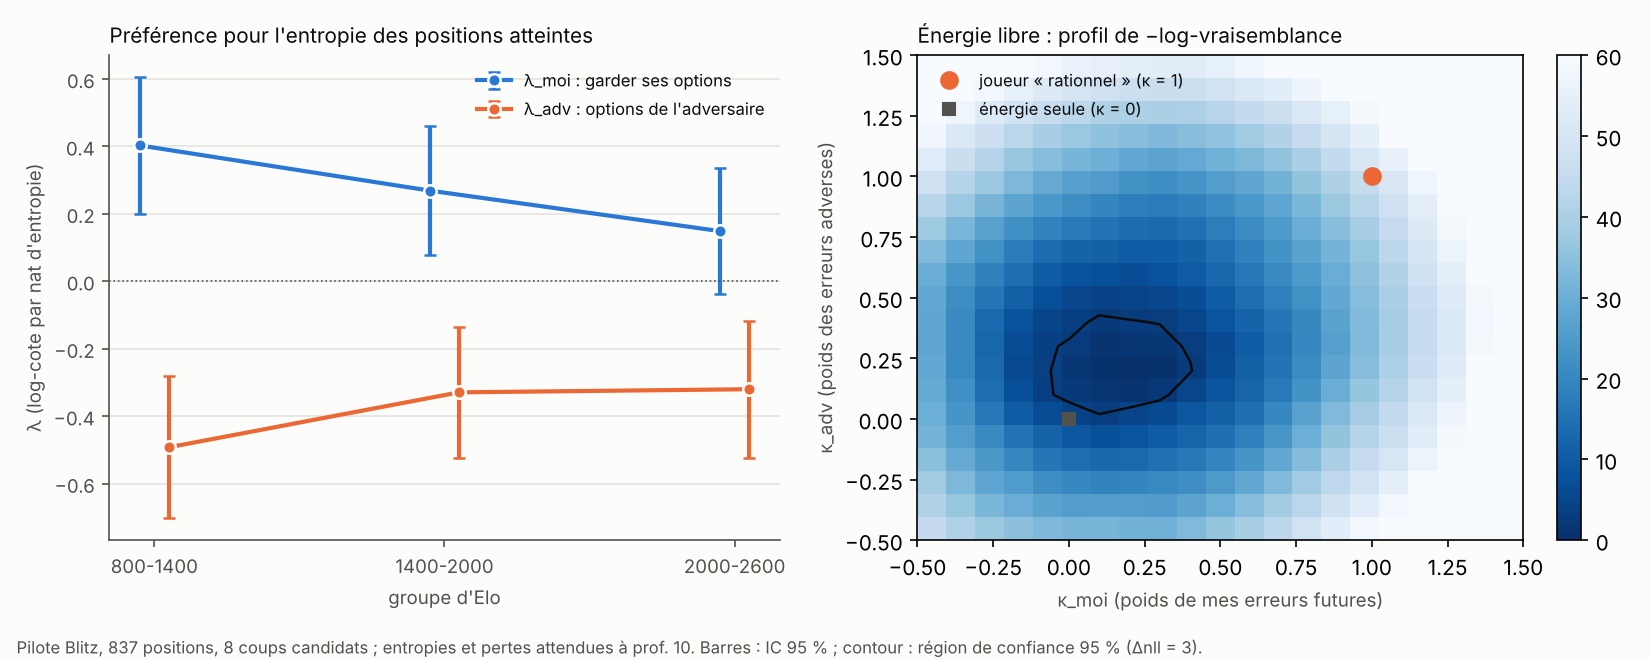
\includegraphics[width=\linewidth]{entropy.png}
  \caption{Gauche : préférences entropiques par niveau ($\lambda_\text{moi}>0$ : garder ses options ;
  $\lambda_\text{adv}<0$ : priver l'adversaire des siennes). Droite : profil de vraisemblance du modèle B ;
  le minimum est loin du point $\kappa=1$.}
\end{figure}

\paragraph{Liens avec les pistes précédentes.}
Le joueur qui mène \og simplifie\fg{} (piste 3) : c'est une réduction d'entropie, à tester directement avec
$\lambda$ selon le score. La chaleur spécifique (§6) montre que les positions où un coup se détache discriminent les
niveaux ; $S_\text{adv}$ faible fabrique précisément ce type de position pour l'adversaire. Enfin, la préférence pour
les options pourrait faire partie de la \emph{saillance} de l'étage 1 du modèle à deux étages (§4).

\paragraph{Limites du pilote.} 837 positions, Blitz seulement ; entropies mesurées à profondeur 10 ; meilleure
réponse adverse supposée pour $S_\text{moi}$ ; seuil de 50 cp arbitraire (à faire varier). Extension complète :
$\sim$9000 positions, $\approx$ 3 h de calcul.
